\part{Week 2}
\chapter{Overview of Quantum Computing}

\section{Global Perspectives}
We'll first look into how QIC originated, how different fields like quantum physics, computer science, information theory, cryptography have contributed in it's development. No one would've thought we could process information and do computing using quantum mechanical systems few decades ago.
\subsection{History of QIC}
It all began in the turn of twentieth century, when the "then physics", now known as classical physics resulted in absurdities. Like ultraviolet catastrophe, involving infinite energies and the well known electron spiralling into nucleus in around $10^{-8}$ seconds. Small changes were made everytime, until it resulted in the modern theory of \textit{quantum mechanics} after like a quarter of century. Now it's used in a wide range of fields from structure of DNA to semiconductors to study of nuclear fusion in stars.

\textit{Quantum Mechanics} is a mathematical framework or a set of rules which base our physical theories. For example \textit{quantum electrodynamics} is a fantastic theory built within the framework of quantum mechanics which describes the interaction between atoms and light. It contains it's own set of rules. The rules of quantum mechanics are simple, but even experts found them counter intuitive, one of the main aim of QIC is to build tools which sharpen our intuition of quantum mechanics.

For example, the problem of signalling faster than light, impossible according to Einstein. In quantum mechanics, it converted into the problem whether we \textit{clone} (make a copy of) a quantum state. Even though it is possible in classical mechanics, the \textit{no-cloning} theorem was proved in quantun mechanics. Few imperfect cloning devices were developed which helped us understand it more.

A historical thing which led to the development of QIC is problem of obtaining \textit{complete control over single quantum systems}. The way we used quantum mechanics then had control over a large composite of quantum systems. For example, we could explain superconductivity incredibly well, but we had control over a huge bunch of atoms (quantum systems) to explain that. Slowly, few methods were developed, like isolating an atom by "trapping" it, electron tunnelling microscope which had control over single atoms etc. The reason we tried gaining control over a single quantum system was on a hunch. Most profound insights in science come when we try developing methods to explore new regimes of nature. Famous examples are radio astronomy, low temperature physics etc. In a similar way, there is a hope of discovering new phenomena if we have control over a single quantum system. QIC fits naturally in this problem. A deep understanding and the ability to harness the powers of QIC is essential to gain control over a single quantum system. Despite these efforts, quantum information processing systems have seen modest success, what we can do now is a dozen of operations on few qubits, few real world applications of \textit{quantum cryptography}. It's a challenge now to develop computational methods to take it to a large scale. 

Another big field, a great intellectual triumph, which contributed to QIC is \textit{computer science }. It's history roots back to very old times. But the proper modern incarnation of computer science was announced by \textit{Alan Turing}. \textit{Turing} developed an abstract notion of what we now call as a programmable computer, the \textit{Turing machine}. He also developed the notion of \textit{Universal Turing machine} which could simulate any other turing machine. Another pioneer of computer science, \textit{Alonzo Church}, developed \textit{Church-Turing} thesis, which says if an algorithm can be done on any physical device, an equivalent algorithm is present for a Turing machine, which does the same task. He developed rigorous mathematicalental concepts which are equivalent to what class of algorithms that can be performed by a physical device.

Slowly electrical components like transistors started to develop and programmable computers were made. This growth was codified by \textit{Moore's Law}, which states computer power would double for constant cost roughly every two years. But this law would eventually reach it's limits, as the components would shrink to maximum physical limit. Quantum mechanics would start interfering in the functioning of electrical devices. One possible solution to the failure of Moore's law is to move to a different computing paradigm, which is provided by QIC. A classical computer could simulate a quantum computer, but it's impossible to do it \textit{efficiently}, since quantum computers provided way faster speed. Many reasearchers believe that no \textit{conceivable} amount of development of classical computers would bridge the gap between the powers of a classical computer and powers of a quantum computer.

There are algorithms which are \textit{efficient}, i.e in \textit{computational complexity } terms, they can be solved in polynomial time, others are \textit{inefficient algorithms}. An observation was made which was codified into \textit{strengthened Church-Turing} thesis:-
\begin{center}
    \textit{Any algorithmic process can be simulated effectively using a turing machine.}
\end{center}
But when \textit{analog} computers were developed, theoretically they could solve few problems efficiently which couldn't be efficiently solved by a Turing machine, violating the aforementioned strengthened church-turing thesis. But realistically , considering the noises these couldn't solve the problems efficiently which turing machine couldn't solve efficiently. This consideration of noise was challenge in the development of QIC, which led to theories of \textit{quantum error-correcting codes} and \textit{fault-tolerant quantum computation}. Thus, quantum computers can tolerate a finite amount of noise while having the computational edge.

A major challenge faced by the Church-Turing thesis is when Robert Solovay and Volker Strassen showed that it is possible to find whether an integer is prime or not using a \textit{randomized algorithm}. This could just determine whether a number is \textit{probably} prime or composite with a \textit{certainty}.  At that time, no deterministic primality algorithm was known, neither is now. Hence this suggested that there are efficiently solvable problems which can't be solved efficiently using a deterministic Turing machine. Hence, the strengthened Church-Turing thesis was changed to

\begin{center}
    \textit{Any algorithmic problem can be stimulated efficiently using a \textbf{probabilistic} turing machine.}
\end{center}

This kind of \textit{ad hoc} modification meant that in future there could be some other computational model found which could solve problems efficiently which couldn't be solved efficiently by a Turing machine. Motivated to find a computational model which could simulate any other model of computation, In 1985, David Deutsch tried to look for physical theories which could be a foundation for Church-Turinh thesis which would be as secure as the physical theory, it should simulate any \textit{arbitrary} physical system. Since all laws of physics are ultimately quantum mechanical laws, he considered devices based on principles of quantum mechanics, which were the quantum mechanical analogues of machines defined by Turing, forty-nine years earlier, which now we're considering as a quantum computer.

We still don't surely know whether Deutsch's notion of Universal quantum computer could solve any probleme efficiently. Maybe some mew strange effect from esoteric theories like quantum field theory, string theory, quantum gravity etc. might open a new dimension of computational models, which could solve problems not efficiently solvable by Deutsch's model. Still Deutsch gave a challenge to Church-Turing thesis. Slowly for few problems like finding prime factors of an integer and 'discrete logarithm' problem, it was shown that quantum computing is way superior to classical computing, as it provided an efficient solution while the latter couldn't. It's not possible to simulate quantum mechanical systems on a classical computer, while it is possible on a quantum computer, a problem with profound scientific and technological implications solved.

Coming up with good quantum algorithms which a quantum computer would solve more quickly than a classical computer is difficult. A pessimist might think it's because quantum computers can solve only the problems which have been discovered yet.  But the actual reasons for why designing algorithms for quantum computers are \begin{enumerate*}[label=(\alph*)]
    \item Human intuition is rooted in the classical world, when we use that intuition to construct  algorithms, they'll  be based on classical idea, whic wouldn't use true quantum effects to achieve a good quantum algorithm. Thus we have to turn off our classical intuition while designing quantum algorithms.
    \item  It's not enough to merely design a quantum mechanical algorithm, we have to make it \textit{better} than any exisiting classical algorithm! for which we have to make use of true quantum aspects of quantum mechanics, which isn't a widespread interest because classical algorithms with comparable performace characteristics exist.
\end{enumerate*}
This makes designing quantum algorithms a challenge!

Let's now change our focus to another big contributor to quantum computation and quantum information, information theory. In 1948, Claude Shannon laid the foundation of modern information and communication theory through his papers. The key step taken by Shannon was \textit{to mathematically define the concept of information.} There are \textit{different ways} to define fundamental things like this, which might have their widespread use. But the definition by Shannon is by far the most fruitful in terms of better understanding, a plethora of deep results and a theory with a rich structure which seems to reflect many (not all) real-world communication problems.

Shannon was interested in two key questions which he answered by proving the two fundamental theorems of information theory. Them being
\begin{enumerate*}[label=(\alph*)]
    \item what resources are required to send information reliably over a communication channel? Shannon's first theorem, \textit{noiseless channel coding theorem}, quantifies the physical resources needed to store the output from an information source.
    \item can information be transmitted while being protected against the noises in the communication channel? Shannon's second theorem, \textit{noisy channel coding theorem}, quantifies how much information is possible to reliably sent over through a noisy channel.
\end{enumerate*}
To achieve reliable transmission in presence of noise, Shannon showed that \textit{error-correcting codes} could be used to protect the information. He gave the upper limit of protection it can give, but doesn't give the limiting codes. Many error-correcting codes are being researched and contructed these days, which are reliable enough to be used for computer modems, satellite systems etc. Do not that this is all classical physics.

Quantum information theory followed similar developmenet. First, Ben Schumacher provided an analogue to noiseless channel coding theorem, and defined a 'quantum bit' or 'qubit' as a tangible physical resource. However, no anallogue of noisy channel coding theorem is known till now. However their counterparts have been developed, as theory of quantum error correction, allowing quantum computers to effectively compute in presence of noise, also allowing transfer of data over \textit{noisy quantum} channels effectively. Classical ideas of error-correction have been important in understanding quantum error-correction codes. Slowly, an important class of codes, CSS codes were developed. These were then subsumed \textit{stabilizer codes}, these were felicitated by a deep understanding of classical linear coding theory.

Theory of quantum correcting codes was developed to protect quantum states, against noise, but if we tried to transmit \textit{classical} information, few surprises were found. Like two classical bits of information being transferred by a single qubit, known as \textit{superdense coding}. Another example, \textit{distributed quantum computation}, where we consider two communicating quantum computers, in certain problems, these would take \textit{exponentially lesser time} compared to classical computers connected. But these problems are of little practical application and have technical restrictions, which is a challenge in front of us.

There's also a \textit{networked information theory} which deals with communications with network of many channels. There's not much known about the networked information theory, but the theory is very valuable and gaining insights into it would open up a lot of new things. For example, we have Alice and Bob, they want to send information through a noisy quantum channel which has zero capacity for quantum information. No information is possible to be communicated between them. But suppose we have two such channels operating synchronously, they still have zero capacity. But if we reverse one of the channels, then according to quantum mechanics, this network has non-zero capacity and we can transfer information between them.

\begin{figure}[h]
    \centering
    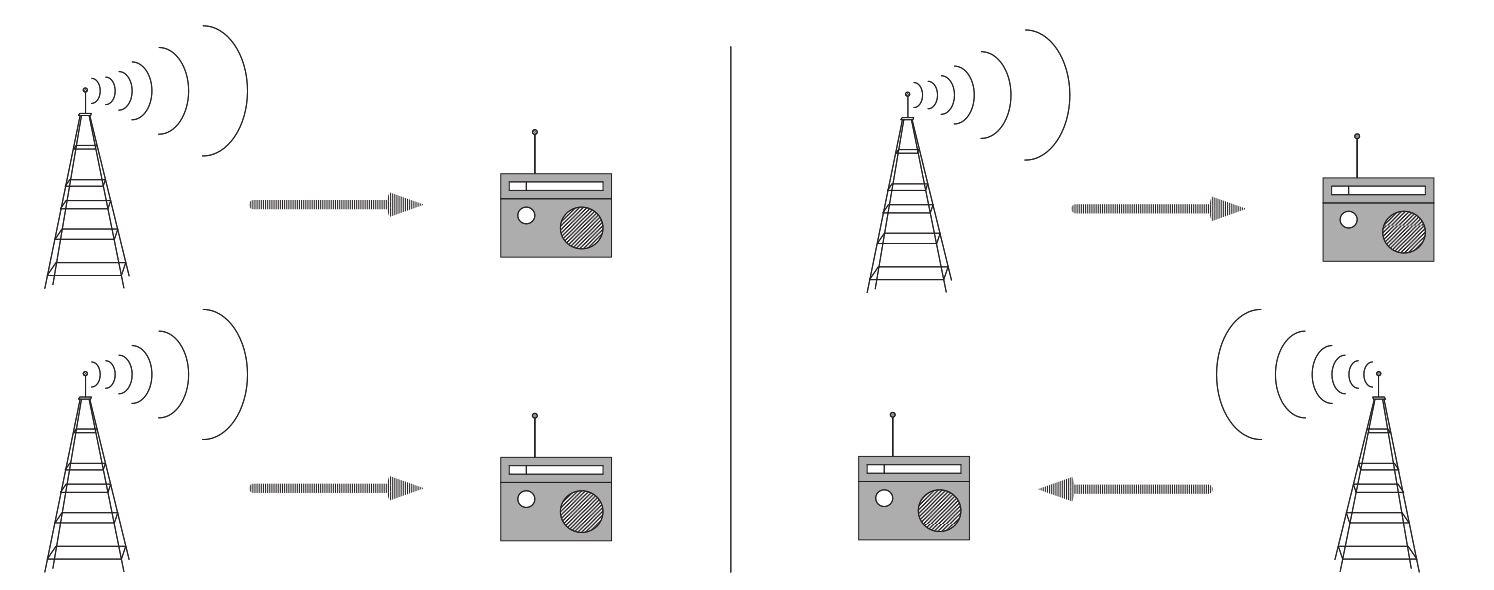
\includegraphics[width=\textwidth]{images/reversing.png} 
    \caption{Reversing one of the channel makes the channel have a non-zero capacity}
    \label{fig:reversing}
\end{figure}

Let's finally move to the respected old art and science of \textit{cryptography}. It's broadly described as the \textit{communication} between two parties \textit{who may not trust each other}. An important case for cryptography is when one party wants to send a secret message to another, without anyone eavesdropping. This is done through a \textit{cryptographic protocol}. Two main ways this can be done is through \begin{enumerate*}
    [label=(\alph*)] \item \textit{public key cryptosystems} \item \textit{private key ecosystems}
\end{enumerate*}.

In \textit{private key cryptosystems}, both party share a private key initially, using which they send \textit{encrypted} messages to each other. Hence only these two can \textit{decrypt} the message, no one else. But the main problem of this is, how are the private keys distributed? what if a third person eavesdrops while they're being distributed? He can get to know every secret message between them. An early discovery of QIC solves this, using \textit{quantum cryptography} or \textit{quantum key distribution}. The basic idea used from quantum mechanics is that if an eavesdropper tries to measure the private key when Alice and Bob are distributing it, they can see that the state of communication channel has changed. Hence they get to know someone's out there and restart it. 

In \textit{public key cryptosystems}, each party makes it's own 'public key', which is made \textit{available to the genreal public}. Using this key of Bob, Alice can encrypt the message. For a third person, it's \textit{extremely difficult} to decrypt this. Not even Alice can decrypt this in real time. Only Bob, who has the keys to his public key personally, can decrypt it. This is most popular these days. The encryption is done through \textit{RSA cryptosystem}. The key here is, it should be extremely decrypt the encryption only with the public key. For this, RSA uses something closely similar to factoring. But Shor's algorithm, run on a quantum computer can to this effectively. Few use discrete logarithm problem, which can also be done effectively by Shor's algorithm. This implies a need of quantum computing and quantum information.

The most striking of these in the study of \textit{quantum entanglement}. It is a unique quantum mechanical \textit{resource} which plays a key role in many applications of QIC. It's like iron to the classical world's bronze age. There's no proper theory of quantum entanglement as of now, a lot of effort is being made. Further study of quantum entanglement is going to lead to amazing new discoveries in quantum computation \subsection{Measurement in bases other than the computational basis}
If we try to represent the state of a system $\qv = \alpha \qo + \beta \qi$ in a different basis, $\ket{a}$ and $\ket{b}$, which are \textit{orthonormal}, we can write it as $\alpha'\ket{a}+\beta'\ket{b}$. According to the postulates of quantum mechanics, if we try to measure with respect to the basis $\ket{a}, \ket{b}$, we get \textit{a} with probability $|\alpha'|^2$ and \textit{b} with probability $|\beta'|^2$. We will learn more about the efficiency of measuring with respect to a basis in further study. of $\qo$ and $\qi$ as \begin{equation}
    \qv = \alpha \qo + \beta \qi,\ \alpha,\beta \in \mathbb{C}
\end{equation}
$\qo, \qi$ are known as \textit{computational basis states}. Unlike a classical bit, we can't determine state of a qubit. When we try observing/measuring it, we get $\qo$ with probability $|\alpha|^2$ and $\qi$ with probability $|\beta|^2$. Thus $|\alpha|^2 + |\beta|^2 = 1$. Hence we can think of the state as unit vector in a complex vector space with the computational bases. This unobservablity of a qubit makes up the heart of QIC. 

A state $\qv$ of a qubit can be represented as,
\begin{equation}
    \qv = e^{i\gamma}\left( \cos{\frac{\theta}{2}}\qo + e^{i\varphi}\sin{\frac{\theta}{2}}\qi  \right)
\end{equation}
which equal to this by a global factor $e^{i\gamma}$,
\begin{equation}
    \qv = \cos{\frac{\theta}{2}}\qo + e^{i\varphi}\sin{\frac{\theta}{2}}\qi
\end{equation}
$\theta, \varphi$ define a point on a sphere known as the \textit{Bloch sphere}; this thing describes many operations of qubits properly. But this doesn't generalize when it comes to multiple qubits.
\begin{figure}[H]
    \centering
    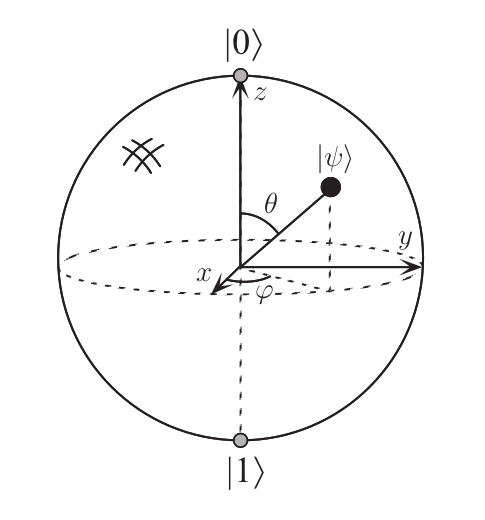
\includegraphics[width=0.5\textwidth]{images/bloch_sphere.png}
    \caption{Bloch sphere representation of a qubit.}
    \label{fig:bloch_sphere}
\end{figure}

\subsection{Multiple qubits}
State vector $\qv$ of a system of two qubits can be defined as,
\begin{equation}
    \qv = \alpha_{00} \ket{00}
         +\alpha_{01} \ket{01}
         +\alpha_{10} \ket{10}
         +\alpha_{11} \ket{11}
\end{equation}
It can be seen that it has four \textit{computational bases}, $\ket{00}, \ket{01}, \ket{10}, \ket{11}$. Even here when we measure the qubit, we get $x=(00, 01, 10, 11)$ with probability $|\alpha_x|^2$ and the qubit collapses to the state $\ket{x}$. By \textit{normalization}, $\sum_{x\in \{0,1\}^2} |\alpha_x^2| = 1$, where $\{ 0, 1\}^2$ is set of all strings with each character 0 or 1. For this set of two qubits, if we try to measure a subset of this, i.e a qubit, say first qubit, the probability of getting the output 0 is $|\alpha_{00}|^2+|\alpha_{01}|^2$ and after measuring, the system collapses to
\begin{equation}
    \ket{\psi'} =
    \frac{\alpha_{00} \ket{00}
         +\alpha_{01} \ket{01}}{\sqrt{|\alpha_{00}|^2+|\alpha_{01}|^2}}
\end{equation}
This is a similar collapse \textit{re-normalized} with a normalization constant.

Another interesting thing can be seen if we consider the Bell state,
\begin{equation}
    \qv = \frac{\ket{00}+\ket{11}}{2}
\end{equation}
If we try to measure $\qo$, we get the output 0 with probability $\frac{1}{2}$ and the bell state collapses to $\ket{00}$, and the output 1 with probability $\frac{1}{2}$ with the bell state collapsing to $\ket{11}$. We can see that if we get 0 we perfectly know about second qubit, i.e measurements are \textit{correlated}. Also, a set of $n$ systems can store $2^n$ amount of information, even though when we measure it, it collapses.

\section{Quantum Computation}
Similar to an electrical circuit, there's a \textit{quantum circuit} which performs operations on qubits using \textit{quantum gates}.
\subsection{Single qubit gates}
We can think of a \textbf{not} gate similar to it's classical analogue, which converts $\qo$ to $\qi$  and vice-versa. It's also linear, i.e \textbf{not} gate when acted on the state
\begin{equation}
    \alpha\qo + \beta\qi
\end{equation}
it interchanges $\qo$ and $\qi$ to give
\begin{equation}
    \alpha\qi + \beta\qo
\end{equation}
This fact is very important, which can be realised later. \textsc{not} gate can be represented by the matrix
\begin{equation}
    X \equiv \begin{bmatrix}
        0 & 1 \\ 1 & 0
    \end{bmatrix}
\end{equation}
For a matrix $U$ to be a \textit{quantum gate}, it has to be unitary and this is the \textit{only} constraint.

Few interesting gates are $Z$, which leaves $\qo$ unchanged while flips the sign of $\qi$,
\begin{equation}
    Z \equiv \begin{bmatrix}
        1 & 0 \\ 0 & -1
    \end{bmatrix}
\end{equation}
The output is equal upto a relative phase factor, the other is the \textit{Hadamard gate}, H given by
\begin{equation}
    H \equiv \frac{1}{\sqrt{2}}\begin{bmatrix}
        1 & 1 \\ 1 & -1
    \end{bmatrix}
\end{equation}
\begin{figure}[H]
    \centering
    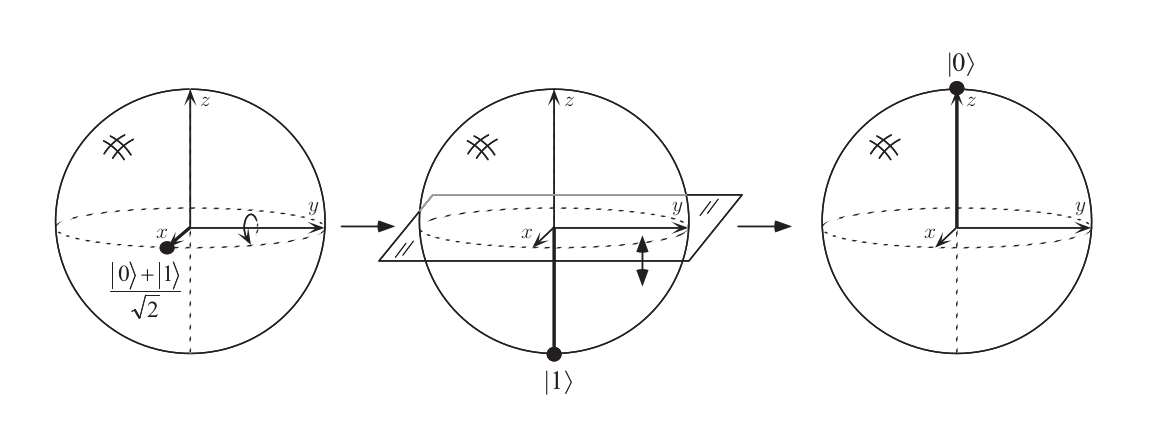
\includegraphics[width=\textwidth]{images/hadmard_bloch.png}
    \caption{Hadmard gate acting on $\frac{\qo + \qi}{\sqrt{2}}$ to give $\qo$}
    \label{fig:hadmard_bloch}
\end{figure}
This get takes $\qo$ to $\frac{\qo + \qi}{\sqrt{2}}$ and $\qi$ to $\frac{\qo-\qi}{2}$. In the Bloch sphere point of view, this rotates the sphere first w.r.t $\hat{y}$ axis by $90^\circ$ and then rotates w.r.t $\hat{x}$ axis by $180^\circ$.

These qubit gates are summarised as
\begin{figure}[H]
    \centering
    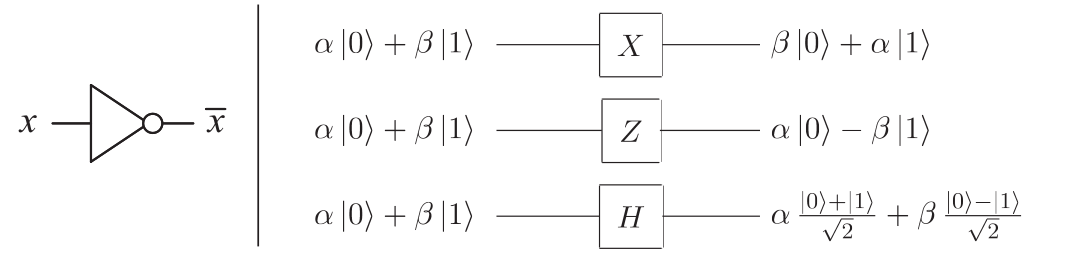
\includegraphics[width=\textwidth]{images/qubit_gates.png}
    \caption{Single bit (left) and Qubit (right) logic gates.}
    \label{fig:qubit_gates}
\end{figure}
We can see that any unitary matrix corresponds to a single qubit gate. Since, there are infinitely many unitary matrices, there are infinitely many single qubit gates. But we can represent this set only with a few single qubit gates. It can be shown that any unitary matrix  $U$ can be written as
\begin{equation}
    U = e^{i\alpha}\begin{bmatrix}
        e^{-i\beta/2} & 0 \\ 0 & e^{i\beta/2}
    \end{bmatrix}
    \begin{bmatrix}
        \cos{\frac{\gamma}{2}} & \sin{\frac{\gamma}{2}} \\ \sin{\frac{\gamma}{2}} & -\cos{\frac{\gamma}{2}}
    \end{bmatrix}
    \begin{bmatrix}
        e^{-i\delta/2} & 0 \\ 0 & e^{i\delta/2}
    \end{bmatrix}
\end{equation}
This can be seen as a rotation about $\hat{z}$ axis then a rotation about $\hat{y}$ axis followed by a rotation about $\hat{z}$ axis again and global phase shift. Any single qubit gate can be decomposed into a form like this. Also, any computation on a \textit{finite} number of qubits can be generated by a \textit{finite} set of gates known as the \textit{universal} for quantum computation.

\subsection{Multiple qubit gates}
For classical bits, there are \textsc{and, or, nand, nor, xor} gates. \textsc{nand} gate is considered as the \textit{universal gate} as any function of bits can be constructed using \textsc{nand} gates. \textsc{xor} gate can't do this. There's a special multi-qubit quantum gate, known as \textit{controlled-}\textsc{not} gate or \textsc{cnot} gate, which has a \textit{control qubit} and a \textit{target qubit}. If the control qubit is 0, nothing happens to target qubit, whereas if it's 1, the target qubit is flipped. i.e,
\begin{equation}
    \ket{00} \xrightarrow{} \ket{00}; \ket{01} \xrightarrow{} \ket{01};
    \ket{10} \xrightarrow{} \ket{11}; \ket{11} \xrightarrow{} \ket{10}
\end{equation}
The \textsc{cnot} gate is similar to the \textsc{xor} gate, because it's just doing $\ket{A, B} \xrightarrow[]{} \ket{A, B\oplus A}$, where $B\oplus A$ is just the \textsc{xor} gate, is the sum modulo two. There are no similar generalisations for classical \textsc{xor, nand} because they're \textit{irreversible} or \textit{non-invertible}. Information is lost upon the action of these gates which is irretrievable. \textsc{cnot} and single qubit gates are prototypes for all other gates because of the following \textit{universality} result: \textit{Any multiple qubit gate may be composed from \textsc{cnot} and single qubit gates.} 
\begin{figure}[H]
    \centering
    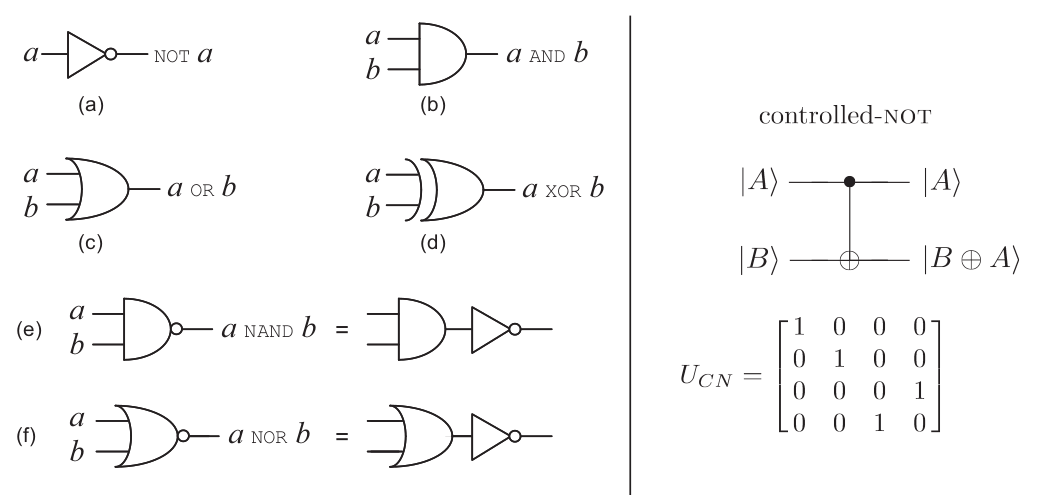
\includegraphics[width=\textwidth]{images/multi_gates.png}
    \caption{Figure on left shows common bit gates; The right figure shows the \textsc{cnot} gate along with it's matrix representation, in the order of $\ket{00}, \ket{01}, \ket{10}$ and $\ket{11}$.}
    \label{fig:enter-label}
\end{figure}

\subsection{Measurement in bases other than the computational basis}
If we try to represent state of a system $\qv = \alpha \qo + \beta \qi$ in a different bases, $\ket{a}$ and $\ket{b}$ which are \textit{orthonormal}as $\alpha'\ket{a}+\beta'\ket{b}$. By postulates of quantum mechanics, if we try to measure w.r.t basis $\ket{a}, \ket{b}$ we get \textit{a} with probability $|\alpha'|^2$ and \textit{b} with probability $|\beta'|^2$. We'll learn more about how efficient is it to measure w.r.t a basis in further study.

\subsection{Quantum circuits}
Similar to classical circuits, quantum circuits are made of wires, which don't necessarily represent physical wires, rather the passage of time or a physical photon moving in space. Let's first look at an example.
\begin{figure}[H]
    \centering
    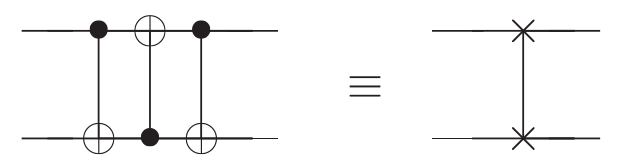
\includegraphics[width=0.5\textwidth]{images/simple_circuit.png}
    \caption{Circuit which swaps two qubits and an equivalent circuit since this is more useful and commonly used.}
    \label{fig:simple-circuit}
\end{figure}
The above circuit swaps two qubits, which can be seen this way considering two qubits with states $\ket{a}$ and $\ket{b}$ as input,
\begin{align}
    \ket{a,b} &\xrightarrow{} \ket{a, b\oplus a} \\
              &\xrightarrow{} \ket{a \oplus (b \oplus a), b \oplus a} = \ket{b, b\oplus a}\\
              &\xrightarrow{} \ket{b, (b\oplus a) \oplus b} = \ket{b, a}
\end{align}
There are few features in classical circuits which aren't seen in quantum circuits. First one is \textit{loops} are not allowed, i.e the circuit is \textit{acyclic}. Second, classical circuit allows joining of wires, an operation known as \textsc{fanin}. Here, the bitwise \textsc{or} operator of inputs is taken. However, information is lost and thus this is irreversible, thus not being allowed in quantum circuits. Thirdly, the inverse of this, where multiple copies of a single bit is made in a classical circuits, known as \textsc{fanout} is not allowed in quantum circuits. We can show that it's impossible to copy a qubit.

There's another important gate, which is in some sense generalisation of \textsc{cnot} gate, \textit{controlled-U} gate. which is represented by this
\begin{figure}[H]
    \centering
    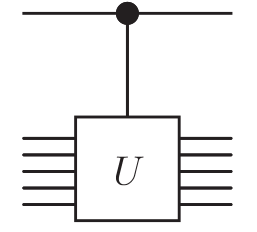
\includegraphics[width=0.2\textwidth]{images/controlled_u.png}
    \caption{Controlled-U gate}
    \label{fig:controlled-u}
\end{figure}
This has similar logic, it's associated with a \textit{unitary matrix} U and takes 1 qubit as the \textit{control qubit}, and $n$ qubits as \textit{target qubits} as inputs. If the control qubit is set to 0, then nothing happens to target qubits. If control qubit is set to 1, then the gate $U$ is applied to all the target qubits. In this sense, \textsc{cnot} gate is the special case when $n=1$ and $U=X$, as shown
\begin{figure}[H]
    \centering
    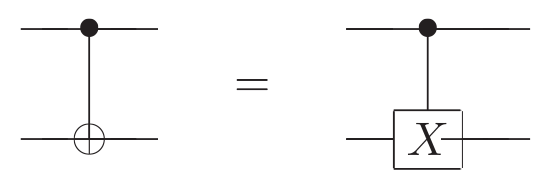
\includegraphics[width=0.5\textwidth]{images/cnot_as_cu.png}
    \caption{Two different representations of \textsc{cnot} gate.}
    \label{fig:cnot-as-cu}
\end{figure}

There's another important operation, known as measurement shown by the 'meter' symbol.
\begin{figure}[H]
    \centering
    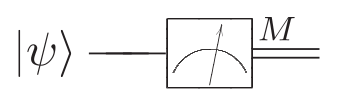
\includegraphics[width=0.4\textwidth]{images/measurement.png}
    \caption{Quantum circuit symbol for measurement.}
    \label{fig:measurement}
\end{figure}
As expected, this outputs a probabillistic classical bit M (which is 0 with probability $|\alpha|^2$ or 1 with probability $|\beta|^2$) if a qubit with state $\qv = \alpha\qo + \beta\qi$ is given as input. Thus, the output is distinguished from a qubit by drawing a double-line wire.

\subsection{Qubit copying circuit?}
First we'll look at a classical example, suppose we have a bit $x$ which we want to copy, we'll use a \textsc{cnot} gate with $x$ and a 'scratchpad bit' 0 as first and second inputs respectively, it'll copy x succesfully as shown
\begin{figure}[H]
    \centering
    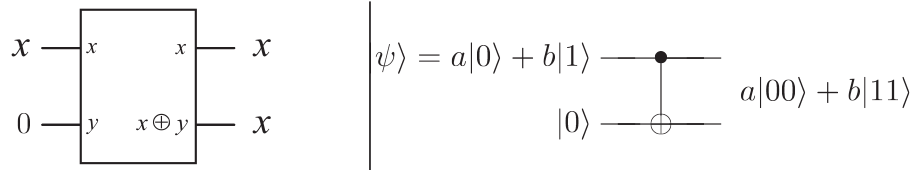
\includegraphics[width=0.8\textwidth]{images/qubit_copy.png}
    \caption{Trying to copy a classical bit (left) and a qubit (right)}
    \label{fig:qubit-copy}
\end{figure}
But if we try copying a qubit with state $\qv = a\qo + b\qi$ in a similar manner using a \textsc{cnot} gate, we can give $\qo$ as an input along with it as
\begin{equation}
    \left[ a\qo + b\qi \right]\qo = a\ket{00} + b\ket{10}
\end{equation}
applying the \textsc{cnot} gate gives $a\ket{00} + b\ket{11}$ as the output. We'd expect the output $\qv\qv$ if we copied $\qv$ succesfully. But that would mean the output should be
\begin{equation}
    \qv\qv = a^2\ket{00} + ab\ket{01} + ab\ket{10} + b^2\ket{11}
\end{equation}
But as we've seen above, it's only possible when $ab = 0$, i.e $a=0$ or $b=0$ i.e we want to copy either $\qo$ or $\qi$. Hence we can't copy $\qv$. It can be shown in general that it is impossible to copy a general qubit with unkown quantum state, if we construct a cloning gate, it can copy different state qubits $\ket{a}$ and $\ket{b}$ only if they are orthogonal. This is known as the \textit{no-cloning} theorem.

There's another way to look at it. An unkown qubit contains some 'hidden' information that isn't directly accessible with a measurement. What's happening above is we get $a\ket{00} + b\ket{11}$, which if we measure we obtain either 0 or 1 using which the other qubit is completely determined. Thus, no extra information is gained. But if we were able to copy $\qv$, then the other qubit contains some more information, contradicting our knowledge, thus a copy can't be created.

\subsection{Example: Bell states}
Let's take a look at a circuit which has a Hadamard gate on first input followed by a \textsc{cnot} gate, as shown
\begin{figure}[H]
    \centering
    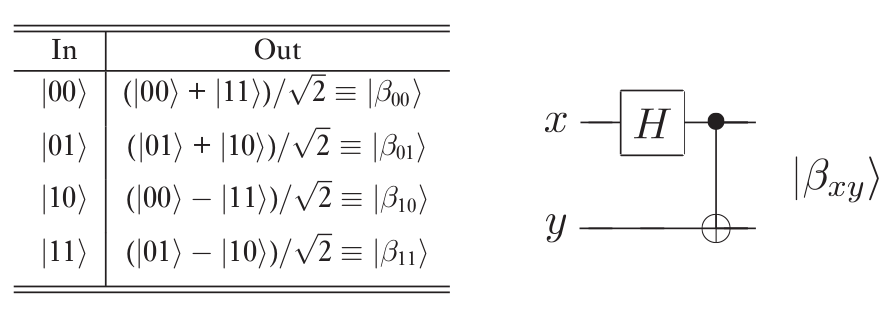
\includegraphics[width=0.9\textwidth]{images/bell_circuit.png}
    \caption{Quantum circuit which creates Bell states, along with it's quantum `truth table'}
    \label{fig:bell-circuit}
\end{figure}
As shown in the truth table, the Hadmard gate first transforms  the first qubit into a superposition after which the \textsc{cnot} gate inverts the target only when control is 1. The output states are
\begin{align}
    \ket{\beta_{00}} &= \frac{\ket{00}+\ket{11}}{\sqrt{2}} \\
    \ket{\beta_{01}} &= \frac{\ket{01}+\ket{10}}{\sqrt{2}} \\
    \ket{\beta_{10}} &= \frac{\ket{00}-\ket{11}}{\sqrt{2}} \\
    \ket{\beta_{11}} &= \frac{\ket{01}-\ket{10}}{\sqrt{2}} 
\end{align}
These are known as the \textit{Bell states} or \textit{EPR states} or \textit{EPR pairs} as their strange properties were found by Einstein, Podolsky and Rosen. Generalizing it,
\begin{equation}
    \ket{\beta_{xy}} = \frac{\ket{0y}+(-1)^x\ket{1\bar{y}}}{\sqrt{2}}
\end{equation}
where $\bar{y}$ is the negation of $y$, $\ket{\beta_{xy}}$ denotes the output when the input given is $\ket{xy}$.

\subsection{Example: quantum teleportation}
It's a non-trivial, surprising and a fun thing! Quantum teleportation is a technique using which we can move quantum states around even in the absence of a quantum communication channel. Consider Alice and Bob, who've met long ago and have shared an EPR pair. Now Alice has a new qubit in state $\qv$ which she doesn't know and has to deliver to Bob. She can only send \textit{classical} information. 

Intuitively, it's pretty bad situation. It's not possible for her to get to know the state $\qv$ completely as she only has one copy of the qubit. Also if she knew the state, it's impossible to transfer this information to Bob, as $\qv$ takes values in \textit{continuous} space, hence requiring infinite amount of time. Quantum teleportation provides a way for it. 

In short, what happens is she measures this state $\qv$ along with the half of her EPR pair. She gets a result in 00, 01, 10 or 11 which she then sends to Bob. Using this information Bob can perform some operations and completely retrieve the state $\qv$ without even getting to know it. Shown using a quantum circuit
\begin{figure}[H]
    \centering
    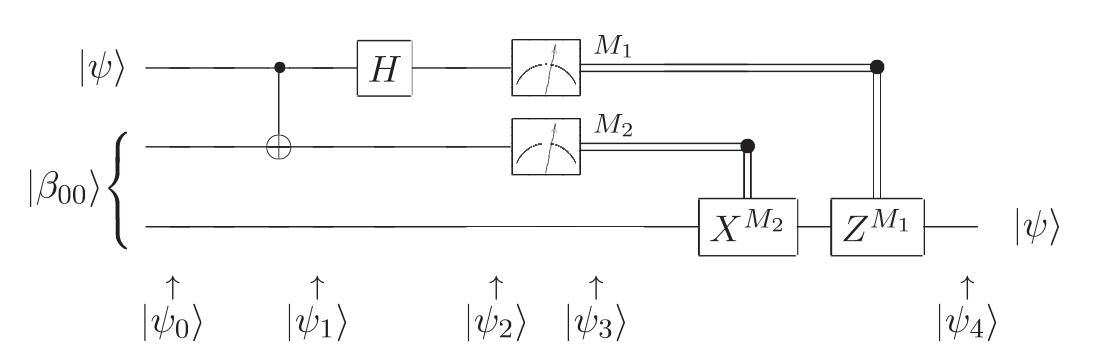
\includegraphics[width=0.8\textwidth]{images/teleportation.png}
    \caption{Quantum circuit showing the teleportation process}
    \label{fig:teleportation}
\end{figure}
Suppose Alice and Bob are sharing $\ket{\beta_{00}}$ and the $\qv$, assuming second input is from alice, overall input to the circuit is 
\begin{align}
    \ket{\psi_0} &= \qv\ket{\beta_{00}} \\
    &= (\alpha\qo + \beta\qi)\left(\frac{\ket{00} + \ket{11}}{\sqrt{2}}\right)\\
    &= \frac{1}{\sqrt{2}}\left[ \alpha\qo\ket{00} + \alpha\qo\ket{11} + \beta\qi\ket{00} + \beta\qi\ket{11} \right]
\end{align}
which when sent through \textsc{cnot} gate on first two qubits gives $\ket{\psi_1}$
\begin{align}
    \ket{\psi_1} &= \frac{1}{\sqrt{2}}\left[ \alpha\qo(\ket{00}+\ket{11}) + \beta\ket{1}(\ket{10}+\ket{01}) \right]
\end{align}
The first qubit is then sent through Hadamard gate, which upon simplifying gives
\begin{align}
    \ket{\psi_2} &= \frac{1}{2}\left[ \alpha(\qo+\qi)(\ket{00}+\ket{11}) + \beta(\qo-\qi)(\ket{10}+\ket{01}) \right]
\end{align}
Now Alice measures the first two qubits of this whole system, giving outputs as $M_1$ and $M_2$ respectively. Based on  what is measured as $M_1M_2$ we can know what is the final state of the qubit Bob has, which is
\begin{align}
    00 &\longmapsto \ket{\psi_3(00)} \equiv \left[ \alpha\qo + \beta\qi \right] \\
    01 &\longmapsto \ket{\psi_3(01)} \equiv \left[ \alpha\qi + \beta\qo \right] \\
    10 &\longmapsto \ket{\psi_3(10)} \equiv \left[ \alpha\qo - \beta\qi \right] \\
    11 &\longmapsto \ket{\psi_3(11)} \equiv \left[ \alpha\qi - \beta\qo \right] 
\end{align}
Now Alice sends these two classical bits to Bob, according to which he knows what kind of transformation to apply on his qubit to transform it to the qubit Alice had. We can verify that he has to apply the matrix $Z^{M_1}X^{M_2}$ to get $\ket{\psi_4}$ i.e $\qv$. Note that the order of matrix multiplication is opposite to the time flow as shown in the circuit diagram.

As we had to transfer classical bits, which can't be done faster than the speed of light, quantum teleportation also can't be done faster than light and is limited by the speed of transfer of the classical bits as faster than light travel could possibly result in sending information backwards in time.

Also note that we haven't created a copy of $\qv$ which would contradict our \textit{no-cloning theorem}. It's because the origin qubit we had in state $\qv$ changes into the state $\qo$ or $\qi$ depending on the value of $M_1$ at the end of the process. Quantum teleportation shows that two classical bits can become a resource at least equal to one qubit information.

\section{Quantum Algorithms}
We'll explore what kind of problems a quantum computer can solve better than a classical computer. How a quantum computer can solve classical problems, we'll also look through well known quantum algorithms.

\subsection{Classical algorithms on a quantum computer}
It turns out that we can simulate any classical circuit using a quantum circuit. It should be possible as physicists believe that everything is explainable using quantum mechanics. We'll kind of prove it in the further discussion. Also, the reason we don't directly use quantum gates to simulate classical gates is that quantum gates are inherently \textit{reversible}, whereas many classical gates such as \textsc{nand} gates are inherently irreversible.

Any classical circuit can be replaced by a reversible elements known as the \textit{Toffoli gate}. Toffoli gate is a reversible gate which takes in three input bits $a,b,c$. If we both the first two input  bits (\textit{control} bits) $a,b$ are 1, it flips the third bit (\textit{target} bit) else it doesn't affect it. It's equivalent to $(a,b,c)\longrightarrow(a,b,c\oplus ab)$ and is represented by this
\begin{figure}[H]
    \centering
    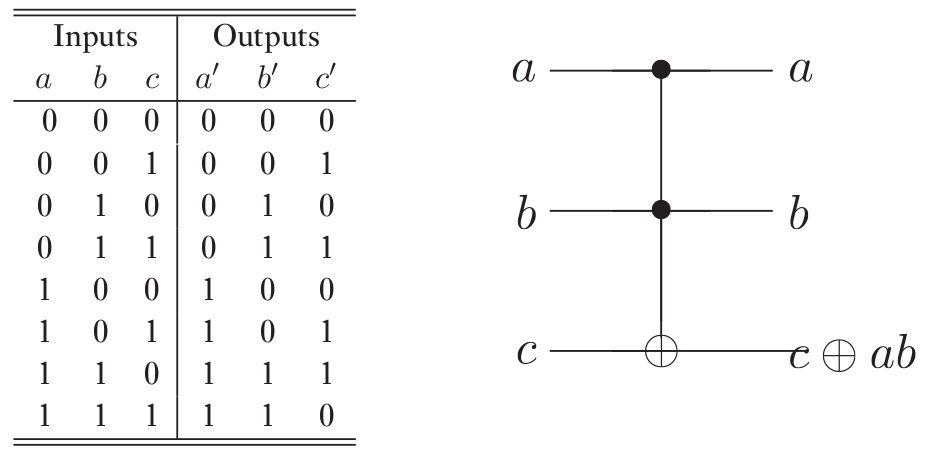
\includegraphics[width=0.7\textwidth]{images/toffoli.png}
    \caption{Left: Truth table for the Toffoli gate, Right: circuit representation of the Toffoli gate.}
    \label{fig:toffoli}
\end{figure}
\begin{figure}[H]
    \centering
    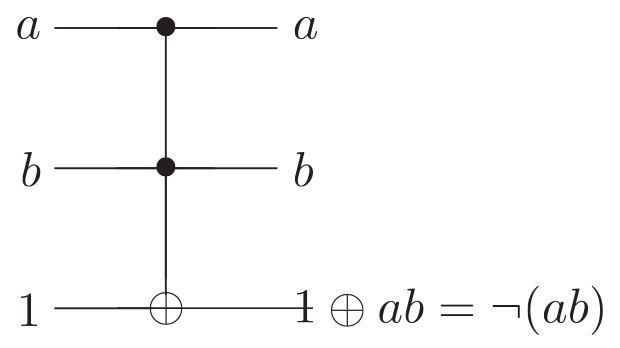
\includegraphics[width=0.4\textwidth]{images/toffoli_nand.png}
    \caption{\textsc{nand} gate simulated using toffoli gate.}
    \label{fig:toffoli-nand}
\end{figure}
\begin{figure}[H]
    \centering
    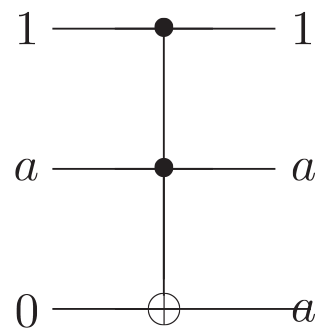
\includegraphics[width=0.2\textwidth]{images/toffoli_fanout.png}
    \caption{\textsc{fanout} gate simulated using Toffoli gate}
    \label{fig:toffoli-gate}
\end{figure}
Toffoli gate can also simulate \textsc{nand} and \textsc{fanout} gates as shown above. Even though we've shown the classical implementation of toffoli gate above, it can be implemented as a quantum logic gate. It works in a similar way as the classical toffoli gate. For example flipping third qubit of $\ket{110}$ to give $\ket{111}$. It can also be proved that this is a valid unitary quantum gate by constructing the corresponding 8 by 8 matrix, $U$. Thus, the quantum toffoli gate can simulate irreversible classical gates, ensuring that quantum computers are capable of what classical computers can do. Not only a classical computer, a quantum computer can simulate a non-deterministic computer, i.e which can generate random bits. A simple way it can do it is preparing a state $\qo$ then applying the Hadamard gate to it, giving $\frac{\qo+\qi}{\sqrt{2}}$ which upon measuring gives $\qo$ or $\qi$ with 50\% probability, thus generating a random number and efficiently simulating a non-deterministic classical computer. A quantum computer is way more advantageous than this and can perform much more powerful functions as we'll discuss further.

\subsection{Quantum parallelism}
\textit{Quantum parallelism} is a fundamental feature of quantum computers. They can evaluate a function $f(x)$ \textit{simultaneously} at many different values. 

Suppose $f:\{0,1\}\xrightarrow{}\{0,1\}$ be a function with a one-bit domain and range. A way of computing this function using a quantum computer is to generate a transform using quantum logic gates which transforms a given state $\ket{x,y} \longrightarrow \ket{x, y\oplus f(x)}$. When $y=0$ the state of the second qubit is just $f(x)$. We name this map as $U_f$ as shown
\begin{figure}[H]
    \centering
    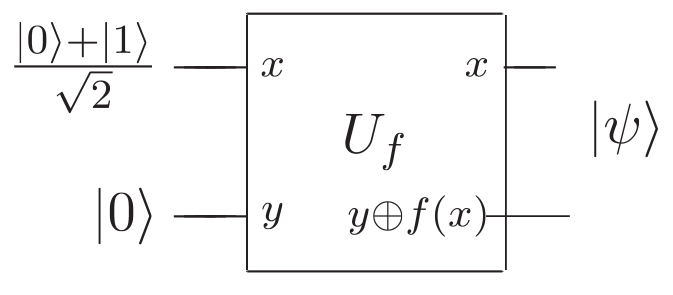
\includegraphics[width=0.6\textwidth]{images/parallelism.png}
    \caption{Quantum circuit for calculating $f(0)$ and $f(1)$ simultaneously. $U_f$ is a quantum circuit which takes $\ket{x,y}$ to $\ket{x, y\oplus f(x)}$}
    \label{fig:parallelism}
\end{figure}
Now if we want to compute both $f(0)$ and $f(1)$ simultaneously, we'll use the superposition state $\frac{\qo + \qi}{\sqrt{2}}$, which can be generated from $\qo$ using a Hadmard gate, and apply $U_f$ on it. We then get
\begin{equation}
    \frac{\ket{0, f(0)}+\ket{1, f(1)}}{\sqrt{2}}
\end{equation}
which contains information about both $f(1)$ and $f(2)$. Thus we've in some sense evaluated both $f(0)$ and $f(1)$ parallely using a single circuit. In classical parallelism, we would have had to construct multiple circuits to evaluate the function at multiple points parallely. We can generalize it to a function which take \textit{multiple} bits as inputs. First we'll apply \textit{Hardmard transform} sometimes known as \textit{Welsh-Hadmard transform} parallely on $n$ qubits. Circuit for $n=2$ is as shown
\begin{figure}[H]
    \centering
    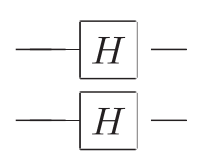
\includegraphics[width=0.3\textwidth]{images/parallel_hadmard.png}
    \caption{Two Hadmard gates ($H^{\otimes 2}$) acting on two qubits parallely.}
    \label{fig:parallel-hadmard}
\end{figure}
For $n=2$ we get
\begin{align}
    \left( \frac{\qo + \qi}{\sqrt{2}} \right) \left( \frac{\qo + \qi}{\sqrt{2}} \right)
    &= \frac{\ket{00}+\ket{01}+\ket{10}+\ket{11}}{2}
\end{align}
This operation can be represented by $H^{\otimes 2}$. For $n$ qubits, as $H^{\otimes n}$. Performing Hadmard transform on $n$ qubits all initialised to $\qo$ gives
\begin{equation}
    \frac{1}{\sqrt{2^n}}\sum_x \ket{x}
    \label{hadmard-eqn-n-qubits}
\end{equation}
Where $x$ is all the possible combinations of $n$ 0's and 1's. 

Now if we want to use quantum parallelism to compute $f(x)$ which takes multi-bit values at multiple values, we first prepare a quantum system of $n+1$ qubits with state $\qo^{\otimes n}\qo$ which upon applying Hadmard transform on first $n$ qubits gives \ref{hadmard-eqn-n-qubits}. This followed by $U_f$ produces
\begin{equation}
    \frac{1}{\sqrt{2^n}}\sum_x \ket{x}\ket{f(x)}
\end{equation}
Do note that we can still \textit{measure} the value of f(x) only at one input. For quantum parallelism to be useful, we need some method to \textit{extract} more informatioin from superposition states like $\sum_x\ket{x}\ket{f(x)}$ .

\subsection{Deutsch's algorithm}
Using this, we can get `global information' about $f(x)$. It combines quantum parallelism with another quantum property known as \textit{interference}. To see how this works, let's create our first qubit as superposition $\frac{\qo + \qi}{\sqrt{2}}$ using Hadmard gate on $\qo$ and our second qubit as superposition $\frac{\qo-\qi}{\sqrt{2}}$ using Hadmard gate on $\qi$. Now let's use this circuit
\begin{figure}[H]
    \centering
    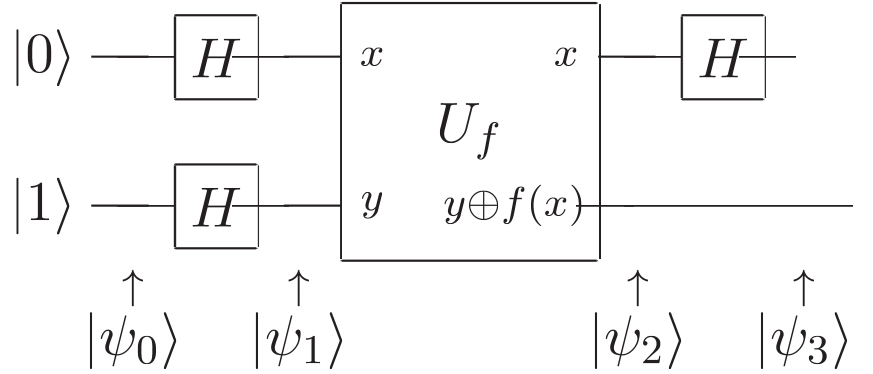
\includegraphics[width=0.7\textwidth]{images/deutsch_algo.png}
    \caption{Quantum circuit implementing Deutsch's algorithm}
    \label{fig:deutsch-algo}
\end{figure}
Our input to this will be
\begin{equation}
    \ket{\psi_0} = \qo\qi
\end{equation}
When Hadmard gates are acted upon them, they become
\begin{equation}
    \ket{\psi_1} = \begin{bmatrix}
        \frac{\qo+\qi}{\sqrt{2}}
    \end{bmatrix}\begin{bmatrix}
        \frac{\qo-\qi}{\sqrt{2}}
    \end{bmatrix}
    \label{eq:U_f_deutsch}
\end{equation}
With a little thought, it can be seen that applying $U_f$ on $\ket{x}(\qo-\qi)/\sqrt{2}$ gives $(-1)^{f(x)}\ket{x}(\qo-\qi)/\sqrt{2}$, Hence applying $U_f$ to $\ket{\psi_1}$ gives
\begin{equation}
    \ket{\psi_2} = \begin{cases}
        \pm\left[
            \frac{\qo+\qi}{\sqrt{2}}
        \right]
        \left[
                \frac{\qo-\qi}{\sqrt{2}}
        \right] &\text{if } f(0) = f(1) \\\\
        \pm\left[
            \frac{\qo-\qi}{\sqrt{2}}
        \right]
        \left[
            \frac{\qo-\qi}{\sqrt{2}}
        \right]&\text{if } f(0) \neq f(1)
    \end{cases}
\end{equation}
Applying the final Hadamard gate on this give $\ket{\psi_3}$
\begin{equation}
    \ket{\psi_3} = \begin{cases}
        \pm \qo \left[ \frac{\qo-\qi}{\sqrt{2}} \right]
        &\text{if } f(0) = f(1)\\
        \pm \qi \left[ \frac{\qo-\qi}{\sqrt{2}} \right]
        &\text{if } f(0) \neq f(1)
    \end{cases}
\end{equation}
This can be condensed more by observing that $f(0)=f(1) \implies 0 = f(0)\oplus f(1)$ and $f(0) \neq f(1) \implies 1 = f(0)\oplus f(1)$, Thus
\begin{equation}
    \ket{\psi_3} = \pm \ket{f(0) \oplus f(1)} \left[ \frac{\qo-\qi}{\sqrt{2}} \right]
\end{equation}
Thus, we can measure $f(0)\oplus f(1)$ by measuring the first qubit. This is really interesting since we found out $f(0)\oplus f(1)$ which is a \textit{global} property of $f(x)$ by just evaluating $f(x)$ \textit{once}! Thus distinguishes a quantum parallelism from even a classical computer. Even a probabilistic classical computer could determine $f(0)$ or $f(1)$ with probability $\frac{1}{2}$ each, a quantum computer evaluates both at once. We can get global information about function by cleverly chosing operation and gates so that the two evaluations \textit{interfere} with each other to give us information like this, which is not possible in classical computers.

\subsection{The Deutsch-Jozsa algorithm}
This is a generalisation to the Deutsch's algorithm. It's application, known as \textit{Deutsch's problem} is described as following. Suppose Alice and Bob are far apart, Alice is in Amsterdam and Bob is in Boston. Alice sends a number $x$ out of $\{ 0,\cdots,2^n-1 \}$ through a letter to Bob. Bob computes a function $f(x)$ which yields the result of either 0 or 1 and mails it back to Alice. Alice needs to find out whether the function $f(x)$ is \textit{constant} or \textit{balanced} i.e 0 for half the values and 1 for the other half by sending as many mails as she can. Using classical means we can figure out that she would need $2^{n-1}+1$ mails to be sent in the worst case.

We can offer a much better solution using qubits if we're sure that Bob is willing to calculate $f(x)$ using a unitary transform $U_f$ in a single interaction. To see how this works, Alice has a set of $n$ qubits each prepared as $\qo$ in which she stores the query $(\sim x)$ and another qubit prepered as $\qi$ where she stores the answer $(\sim f(x))$. She then applies Hadmard transform on all $n+1$ qubits after which she sends these to Bob. Bobs first applies $U_f$ on them and then Alice applies Hadmard transform on the first n qubits such that she gets information about $f(x)$ and thus the solution. We'll look through how this happens. Take a look at the circuit
\begin{figure}[H]
    \centering
    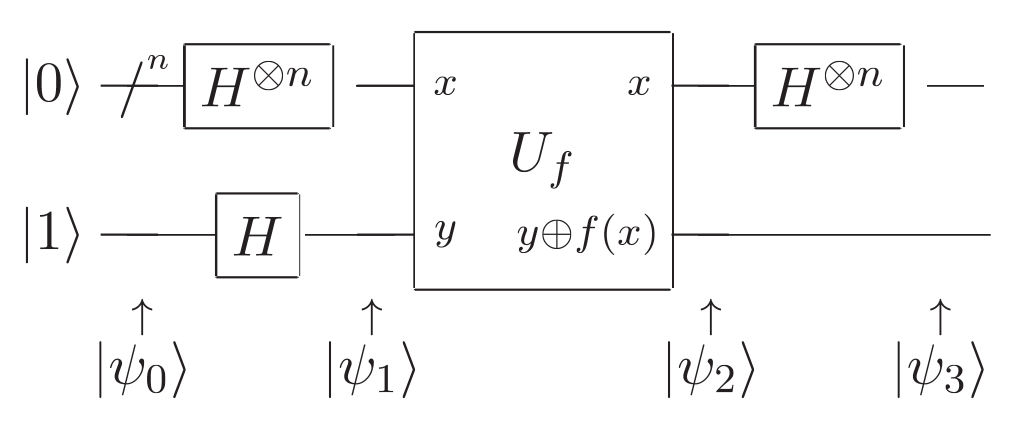
\includegraphics[width=0.7\textwidth]{images/deutsch_jozsa.png}
    \caption{Implementation of Deutsch-Jozsa algorithm, the cross represents $n$ qubits}
    \label{fig:deutsch-jozsa}
\end{figure}
So the input state is
\begin{equation}
    \ket{\psi_0} = \qo^{\otimes n}\qi
\end{equation}
When the Hadmard transform is applied, the query qubits turn into a superposition of $\ket{x}$ where $x$ is binary representation of all numbers in $\{ 0, \cdots, 2^n -1 \}$ 
\begin{equation}
    \ket{\psi_1} = \sum_{x} \frac{\ket{x}}{\sqrt{2^n}} \left[ \frac{\qo-\qi}{\sqrt{2}} \right]
\end{equation}
This is sent to Bob, he applies $U_f$ to $\ket{\psi_1}$ which results in $\ket{\psi_2}$ using similar result as in \ref{eq:U_f_deutsch}
\begin{equation}
    \ket{\psi_2} = \sum_x \frac{\ket{x}}{\sqrt{2^n}}(-1)^{f(x)}\left[ \frac{\qo-\qi}{\sqrt{2}}\right]
\end{equation}
Now comes the tricky part when Alice applies Hadmard gate on first $n$ qubits. Let's just see what happens when Hadamard transform is applied to $\ket{x}$ which is just a binary string (representation of some number $\in \{0,\cdots,2^n-1\}$). We get another superposition of all possible basis states $\ket{z}$ whose quotients are $(-1)^{xz}$ which is bitwise multiplication/\textsc{and} of $x$ and $z$ along with the normalization constant.
\begin{equation}
    H\ket{x} = \sum_z \frac{(-1)^{xz}\ket{z}}{\sqrt{2^n}}
\end{equation}
Thus the final output Alice gets is
\begin{equation}
    \ket{\psi_3} = \sum_x \sum_z \frac{(-1)^{xz+f(x)}\ket{z}}{2^n}\left[ \frac{\qo-\qi}{\sqrt{2}} \right]
\end{equation}
Looking at first n qubits, coefficient of $\qo^{\otimes n}$ turnes out to be just $\sum_x \frac{(-1)^{f(x)}}{2^n}$. Now note that if $f(x)$ was constant $\sum_x(-1)^{f(x)}$ would be $\pm 2^n$, which would mean coefficient of $\qo^{\otimes n}$ is $\pm1$. Since norm of state of a system should be 1 coefficients of all other $\ket{z}$ would be 0. Thus, Alice would only measure $\qo^{\otimes n}$. Now in the case when $f(x)$ is balanced, coefficient of $\qo^{\otimes n}$ would be 0. Hence, Alice would never get the measurement result as 0.
\begin{center}
    \textit{
    Alice gets $\qo^{\otimes n}$ upon measuring $\ket{\psi_3} \iff f(x)$ is constant
    }
\end{center}
Thus by measuring the query register Alice can get to know the answer in just one correspondence. Let's summarise this algorithm

\begin{algorithm}[H]
    \SetAlgoLined\DontPrintSemicolon
    \caption{Deutsch-Jozsa}
    \SetKwInOut{KwIn}{Inputs}
    \SetKwInOut{KwOut}{Outputs}
    \SetKwInOut{KwRun}{Runtime}
    \SetKwProg{myprog}{Procedure}{}{}

    \KwIn{A black box $U_f$ which performs the transformation $\ket{x}\ket{y} \longrightarrow \ket{x}\ket{y\oplus f(x)}$, $x \in \{0,\cdots,2^n-1\}$ and $f(x) \in \{0,1\}$. It's guaranteed that $f(X)$ is either \textit{balanced} or \textit{constant}.}
    \KwOut{0 if and only if $f$ is constant.}
    \KwRun{One evaluation of $U_f$, always succeeds.}
    \myprog{}{
    $\qo^{\otimes n}\qi$ \tcp*{initialize state}\;
    $\longrightarrow \frac{1}{\sqrt{2^n}}\sum_{x=0}^{2^n-1}\ket{x}\left[ \frac{\qo-\qi}{\sqrt{2}} \right]$ \tcp*{create superposition using Hadmard gates}\;
    $\longrightarrow \sum_x (-1)^{f(x)}\ket{x}\left[ \frac{\qo-\qi}{\sqrt{2}} \right]$ \tcp*{calculate $f$ using $U_f$}\;
    $\longrightarrow\sum_z \sum_x \frac{(-1)^{xz+f(x)}\ket{z}}{2^n}\left[ \frac{\qo-\qi}{\sqrt{2}} \right]$ \tcp*{perform Hadmard transform}\;
    $\longrightarrow z$ \tcp*{measure to obtain output}
    }{}
\end{algorithm}

This is a seed for quantum algorithms. But it has it's own problems, such it has no real world application. It can be solved in a more realistic manner using a probabilistic computer.

\subsection{Quantum algorithms summarized}
Broadly speaking, quantum computers are good at solving three classes of problems. First one based upon quantum versions of Fourier transform, Deutsch-Jozsa algorithm, Shor's algorithm and discrete logarithm come under this class. Second class is quantum search algorithms. Third class of algorithms is quantum simulation, using which a quantum computer can simulate a quantum system. Let's look at each of these
\subsubsection{Quantum algorithms based on Fourier transform}
The discrete Fourier transform is described as transforming the set $x_0, \cdots, x_{N-1}$ of N complex numbers into the set of complex numbers $y_1,\cdots,y_{N-1}$ according to this
\begin{equation}
    y_k \equiv \frac{1}{\sqrt{N}}\sum_{j=0}^{N-1} e^{\frac{2\pi ijk}{N}}x_j 
\end{equation}
It's widely known in science because turns a much complex problem into an easier one. There's a more generalized theory of fourier transforms which we won't be discussing. The Hadamard gates we've used in Deutsch-Jozsa algorithm and also the famous Shor's algorithm and discrete logarithm involve some kind of fourier transform. To go into the quantum realm, we can define a linear transform $U$ on $n$ qubits whose action on the basis states $\ket{k}, 0 \leq k \leq 2^n - 1$ is defined as
\begin{equation}
    \ket{j } \longrightarrow \frac{1}{\sqrt{2^n}}\sum_{k=0}^{2^n-1}e^{\frac{2\pi ijk}{2^n}}\ket{k}
\end{equation}
It can be checked that this transform is unitary, and can be realised as a quantum circuit. On a general qubit, this is
\begin{equation}
    \qv = \sum_{j=0}^{2^n-1} x_j\ket{j} \longrightarrow \frac{1}{\sqrt{2^n}}\sum_{k=0}^{2^n-1}\left[\sum_{j=0}^{2^n-1}e^{\frac{2\pi ijk}{2^n}}x_j\right]\ket{k}
    = \frac{1}{\sqrt{2^n}}\sum_{k=0}^{2^n-1} y_k \ket{k}
\end{equation}
Which can be seen as the vector form of fourier transform on the set $x_j$ and $N=2^n$. 

A classical computer would perform the fourier transform in $N\log{N}=n2^n$ steps, whereas a quantum computer would just take $(\log{N})^2=n^2$ steps. Again the same problem arises that a lot of information is "hidden" and not accessible. When we try to measure it the state just collapses to either $\qo$ or $\qi$ making us loose our information. Hence, more cleverness is needed to harness the proper power of quantum computation. We'll come back to more applications of Fourier Transform.

\subsubsection{Quantum search algorithms}
A quantum computer can perform search algorithms, where we have to find an element from a collection of $n$ random elements with a specific property in $\sqrt{n}$ steps. Whereas a classical computer takes $n$ steps. Even though this advantage is less than what we had in fourier transform's case, this field has a wide variety of applications compared to the latter one.

\subsubsection{Quantum simulation}
Simulating quantum system, as expected, is better done by quantum computers than classical ones. For a classical computers the number of complex numbers needed to describe a system grows \textit{exponentially} whereas it grows \textit{linearly} for a quantum computer i.e a quantum system having $n$ components would require $c^n$ bits of memory for a classical computer where c depends on the system and accuracy we need. Whereas a quantum computer would require only $kn$ bits of memory. Again, the $c^n$ bits of information isn't accessible using the $kn$ bit quantum comupter. We'd still just be able to access $kn$ bits of memory. How to extract more information is still partially understood.
Still quantum simulation would be an important applications of QIC as we coould understand about complex chemical molecules which generally occur in biology.

\subsubsection{The power of quantum computation}
We'll try to get some idea of how powerful quantum computers can be compared to classical computers, yet there is still a possibility they are not much powerful than a classical computer. \textit{Computational complexity theory} deals with how difficult can it be to solve a problem. Most basic idea of it is of \textit{complexity class} which is a set of problems all having some kind of similarity in how resource intensive they are.

Two most important complexity classes are \textbf{P} and \textbf{NP}. \textbf{P} is the set of problems which can be quickly solved using a classical computer. \textbf{NP} is the set of problems whose solutions can be quickly checked. For example, there's no algorithm for factoring two integers that's in \textbf{P} on a classical computer. But we can check if $p$ is a factor of $n$, hence it's an \textbf{NP} problem.

It's clear that \textbf{P} is a subset of \textbf{NP} since the ability to solve a problem implies the ability to check potential solutions. But there are no known problems that are "surely" not in \textbf{P} but are in \textbf{NP}. This is a famous open problem in computer science
\begin{equation}
    \textbf{P} \stackrel{?}{\neq} \textbf{NP}
\end{equation}
There's an important subclass of \textbf{NP} problems, known as \textbf{NP}-complete problems. Many hard and highly important problems are known to be \textbf{NP}-complete. In some sense, \textbf{NP}-complete problems are "atleast" as hard as \textbf{NP} problems. Any algorithm solving \textbf{NP}-complete problems can be adapted to solve \textbf{NP} hard problems, with a little overhead. If $\textbf{P}\neq\textbf{NP}$, then there would be no \textbf{NP}-complete problem efficiently solvable by a classical computer.

It is not known whether quantum computers can solve all \textbf{NP} problems. They can solve few problems like factoring which aren't surely known to be in \textbf{NP} but are believed to be in. There's an interesting result that a simple variant of quantum parallelism can't solve all \textbf{NP} problems. But still, this does not rule out that there might be some deeper structure which would let us solve all \textbf{NP} problems on a quantum computer efficiently.

Another important complexity class \textbf{PSPACE} is the set of problems which are efficient on space but not necessarily on time. Even though \textit{not proved}, \textbf{PSPACE} is believed to be bigger than both \textbf{P} and \textbf{NP}. Finally, \textbf{BPP} is the set of problems that can be solved using randomized algorithms with some bound probability error (say 1/4). They're more believed to be the class that can be solved by a classical computer. Even though \textbf{P} is more studied.

\textbf{BQP} is the class  of all computational problems that can be solved efficiently on a quantum computer with a bound probability error. \textbf{BQP} is knownn surely to be bigger than \textbf{P} but not bigger than \textbf{PSPACE}. It's not exactly known where it fits between \textbf{P}, \textbf{NP}, \textbf{PSPACE}.    This gives an important fact that if \textit{quantum computers are strictly powerful than classical computers} then \textbf{PSPACE} is strictly bigger than \textbf{P}. The latter part has been really hard to prove by computer scientists, lowering the hope that quantum computers are more powerful than classical computers.

\begin{figure}[H]
    \centering
    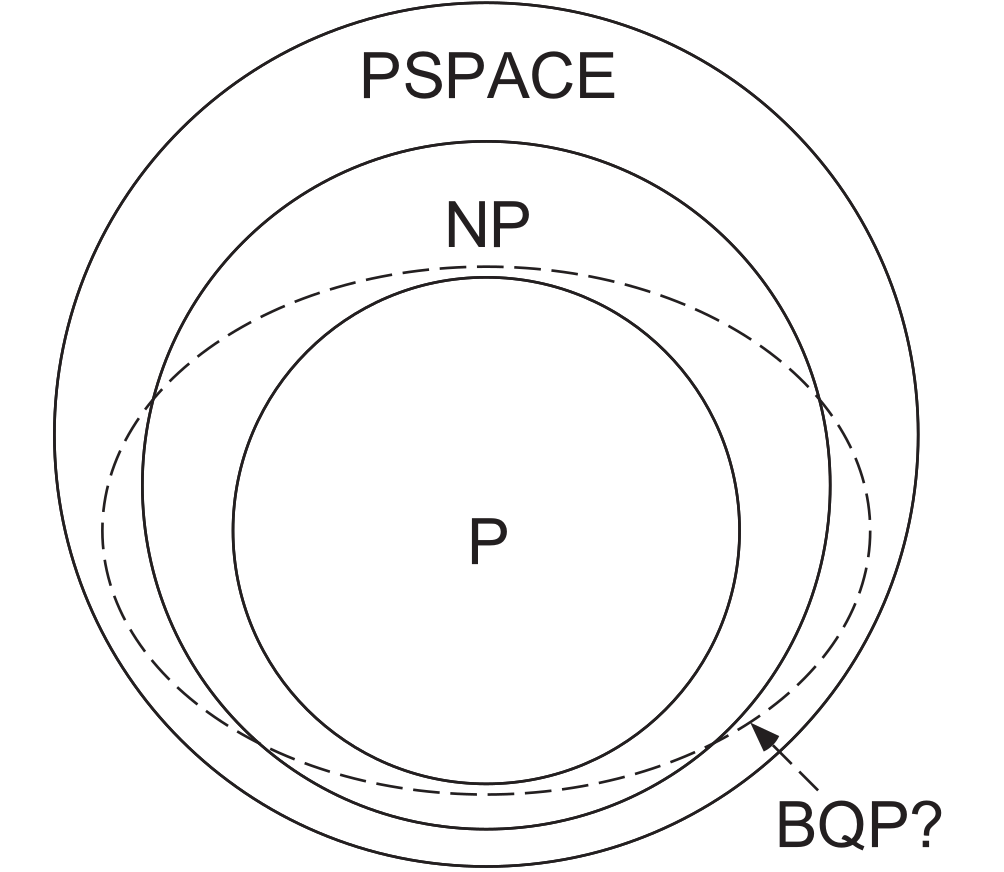
\includegraphics[width=0.6\textwidth]{images/bqp_pspace.png}
    \caption{We surely know that quantum computers can solve all \textbf{P} problems quickly and also that they cannot solve any problem outside \textbf{PSPACE} but we don't know where quantum computers fit between \textbf{P} and \textbf{PSPACE}. We don't even know whether \textbf{P} is equal to \textbf{PSPACE}.}
    \label{fig:bqp-pspace}
\end{figure}
We can already see that the \textit{theory} and notions of quantum computing pose a challenge to traditional computational methods. Another important challenge is that quantum computing is believed to be \textit{experimentally realizable}, primarily because nature works according to quantum mechanics.

\section{Experimental quantum information processing}
We'll look into experimentally proving that quantum computing can be done. Let's start with the "Stern-Gerlach" experiment which provides evidence to the existence of qubits in nature.
\subsection{The Stern-Gerlach experiment}
In the original experiment performed in 1921-22, hot `silver atoms' were beamed from an over through a magnetic field which deflected it. We'll consider the hydrogen atom version performed in 1927 as it's much simpler. A hydrogen atom consists of a proton and an electron spinning around which makes up the atomic dipole moment. By constructing the apparatus properly, it's possible to make the atom deflect by an amount dependent on the $\hat{z}$ component of atomic dipole moment. It's naturally expected that the atomic dipole moments would be randomly oriented and we'd get a continuous distribution. But the atoms were deflecting at specific angles. This was then explained by the \textit{quantization} principle, which was trending at that time. But quantum mechanics had predicted that the net atomic dipole of an atom must be zero, which is classically strange though, but there were two beams seen, one deflected up and the other deflected down.

This puzzle was explained by a new quantity called \textit{spin} which every hydrogen atom is supposed to be associated with. This spin is posited to make \textit{extra contribution} to the magnetic dipole moment.
\begin{figure}[H]
    \centering
    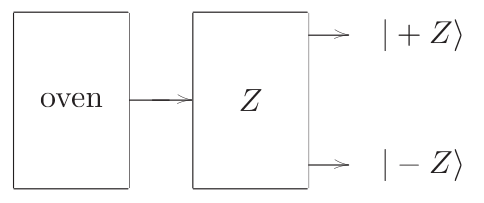
\includegraphics[width=0.4\textwidth]{images/stern_gerlach.png}
    \caption{Original Stern-Gerlach setup.}
    \label{fig:stern-gerlach}
\end{figure}
We can assume that the spins $\ket{+Z}$, $\ket{-Z}$ leads to upper and lower deflection respectively. Now if the apparatus modiied that the upper beam is then passed through another apparatus \textit{tipped sideways} so that it deflects according to $\hat{x}$ axis.

